%%%%%%%%%%%%%%%%%%%%%%%%% User Interaction %%%%%%%%%%%%%%%%%%%%%%%

\section{User interaction}
\label{sec:user-interaction}

In this section we will explain some of the main functionalities
from the point of view of the user by showing different screenshots.
We will focus on 3 actions: ``tagging and sharing an application'', ``locating an
application'' and ``retrieving and adapting and application from the repository''.

\subsection{Tagging and sharing}
Once the user has successfully logged in the system, he can browse the tree to
see all the information related to his applications in the tab ``My
applications'' as is shown in Figure \ref{img:ui-my-applications}. In order to
distinguish quickly between a focus and a nimbus application (see Section
\ref{subsec:intro-awareness-applications}), the applications are presented with a
different icon (cloud for nimbus, glasses for focus) depending on the type.

\begin{figure}[h!]
 \begin{center}
 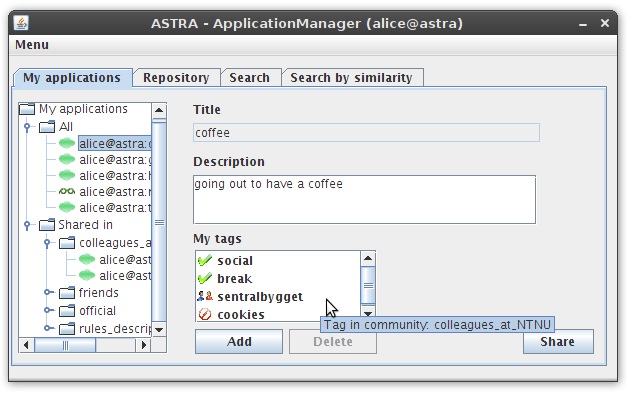
\includegraphics[scale=0.6]{screenshots/ui-my-applications.png}
  \caption{\label{img:ui-my-applications}Interaction with ``My applications''
  (screenshot)}
 \end{center}
\end{figure}

He can manage the tags associated to every application, deleting them or adding
new ones. To make the GUI more intuitive, they are represented with a different
icon depending on the scope as is shown in Figure \ref{img:ui-my-applications}.
There is also a tool tip for every of them, where the user can see the scope
and the community which belongs to in the case of a community tag.
\newline
When the user decides to add a tag, a new window where the user can customize
the scope appears, as is shown in Figure \ref{img:ui-adding-tags}.

\begin{figure}[h!]
 \begin{center}
 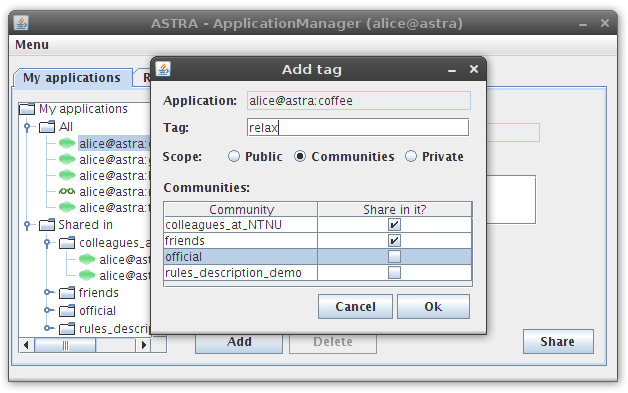
\includegraphics[scale=0.6]{screenshots/ui-adding-tags.png}
  \caption{\label{img:ui-adding-tags}Adding a tag (screenshot)}
 \end{center}
\end{figure}

When the user desires to share an application by pressing the button ``Share'',
another window is displayed. Here he can select the communities where the
application is going to be visible, the rules he wants to share, change the
description, etc. The Figure \ref{img:ui-sharing} shows an screenshot with
that window.

\begin{figure}[h!]
 \begin{center}
 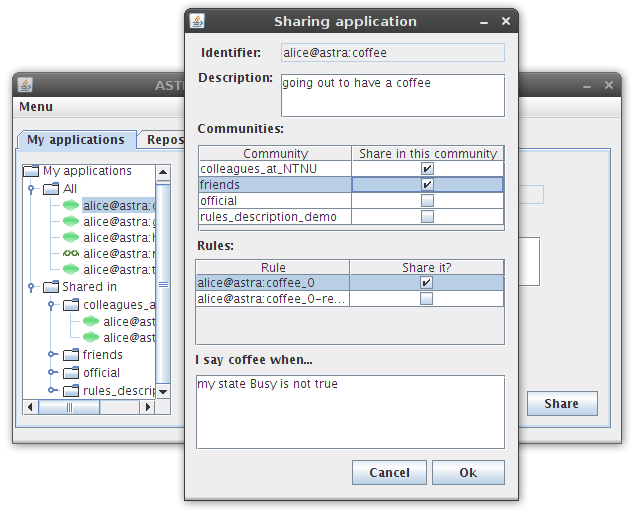
\includegraphics[scale=0.6]{screenshots/ui-sharing.png}
  \caption{\label{img:ui-sharing}Sharing an application (screenshot)}
 \end{center}
\end{figure}


\subsection{Locating an application in the repository}
\label{subsec:ui-locating}
There are three different ways to locate an application in the repository.
The first one is offered in the tab ``Repository'', where the user can browse
the repository and see the main information (description, associated
 visible tags, etc) of the applications which are within his scope. The Figure
 \ref{img:ui-repository} shows the interaction through this tab.
 
\begin{figure}[h!]
 \begin{center}
 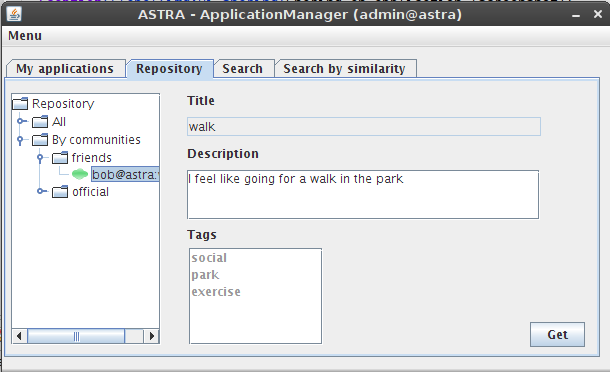
\includegraphics[scale=0.6]{screenshots/ui-repository.png}
  \caption{\label{img:ui-repository}Browsing the repository (screenshot)}
 \end{center}
\end{figure}

The second one is by performing a query, clicking on the tab ``Search''.
Here the user has to select the criteria (any, by description, by tags or by type),
type a query (in natural language, using keywords, etc.) and press the button
``Go!''. Then the results appear in the list below sorted by score, and the
user can see the information related to that results by clicking on them. The
Figure \ref{img:ui-searching-criteria} shows an screenshot of the interaction
through this tab.

\begin{figure}[h!]
 \begin{center}
 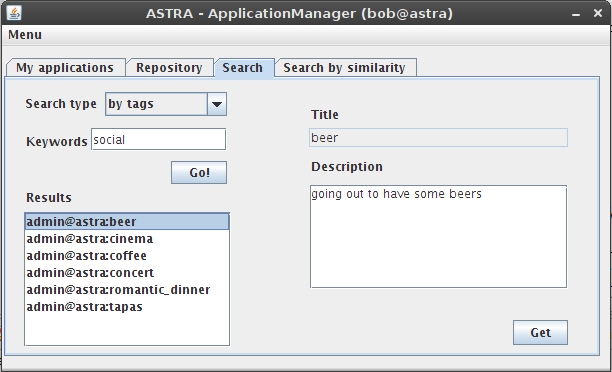
\includegraphics[scale=0.6]{screenshots/ui-searching-criteria.png}
  \caption{\label{img:ui-searching-criteria}Searching an application by  
  criteria (screenshot)}
 \end{center}
\end{figure}

The last option to locate an application is offered in the tab ``Search by
similarity''. Here the user selects one of his applications, and similar
applications sorted by similarity are loaded on the list on the right. Selecting
one of these applications, the user can see the information related to it. The
Figure \ref{img:ui-searching-similarity} shows the interaction through this tab.

\begin{figure}[h!]
 \begin{center}
 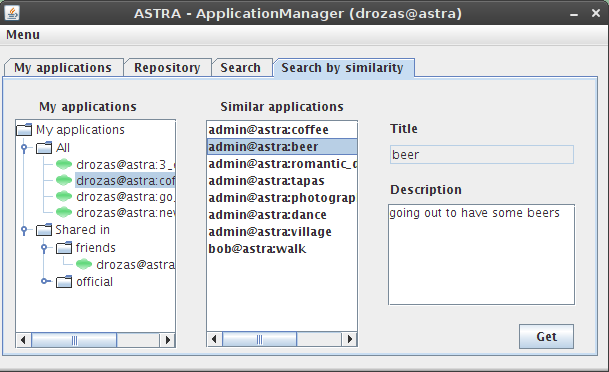
\includegraphics[scale=0.6]{screenshots/ui-searching-similarity.png}
  \caption{\label{img:ui-searching-similarity}Searching an application by 
 similarity (screenshot)}
 \end{center}
\end{figure}

\subsection{Retrieving and adapting an application from the repository}
Once the user has located an application by one of the several ways explained
in Section \ref{subsec:ui-locating} and he decides to get it, a new window
where the user can adapt the application is displayed. He can change the
description and choose the rules he wants to retrieve. The Figure
\ref{img:ui-retrieving} shows an screenshot with the interaction through this
window after having performed a search by similarity.

\begin{figure}[h!]
 \begin{center}
 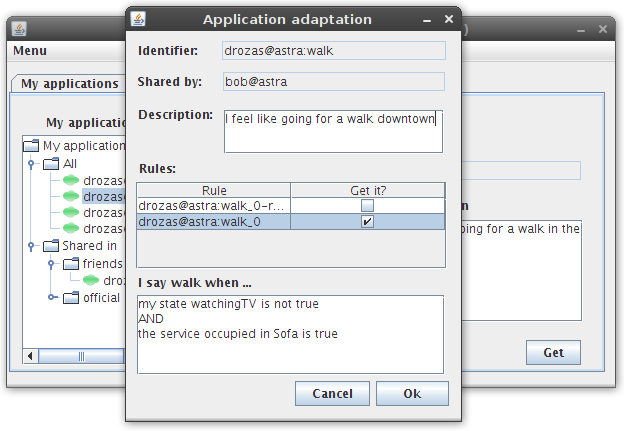
\includegraphics[scale=0.6]{screenshots/ui-retrieving.png}
  \caption{\label{img:ui-retrieving}Retrieving and adapting an application
  from the repository (screenshot)}
 \end{center}
\end{figure}

